\section{角动量守恒}

\begin{wrapfigure}[6]{r}{13em}
  \vspace{-4em}
  \centering
  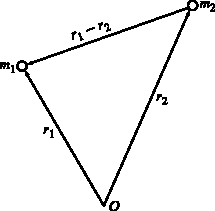
\includegraphics{figure/fig09.01}
  \caption{两质点体系}
  \label{fig:09.01}
\end{wrapfigure}
在这一章里,我们再讨论一种守恒定律。

我们仍然由两个质点构成的孤立体系开始讨论。图\ref{fig:09.01}所表
示的两质点体系,其动力学方程是:
\begin{equation}\label{eqn:09.01.01}
  m _ { 1 } \frac { \dif \vec{v} _ { 1 } } { \dif t } = \vec{F} _ { 2 \to 1 }
\end{equation}
\begin{equation}\label{eqn:09.01.02}
  m _ { 2 } \frac { \dif \vec{v} _ { 2 } } { \dif t } = \vec{F} _ { 1 \to 2 }
\end{equation}
其中$\vec{F} _ { 2 \to 1 }$是质点2对1的作用力;$\vec{F} _ { 1 \to 2 }$
是质点1对2的作用力,没有外力的作用,并且根据牛顿第三第律
\begin{equation}\label{eqn:09.01.03}
  \vec{F} _ { 1 \to 2 } = - \vec{F} _ { 2 \to 1 }
\end{equation}
用矢量$\vec{r} _ { 1 }$ 对式\eqref{eqn:09.01.01}两边进行矢积,得到
\begin{equation*}
  \vec{r} _ { 1 } \times m _ { 1 } \frac { \dif \vec{v} _ { 1 } } { \dif t } = \vec{r} _ { 1 } \times \vec{F} _ { 2 \to 1 }
\end{equation*}
根据矢量的微分法则,上式右边有
\begin{equation*}
  m _ 1 \vec{r} _ { 1 } \times \frac { \dif \vec{v}_ { 1 } } { \dif t } = m _ { 1 } \frac { \dif } { \dif t } ( \vec{r} _ { 1 } \times \vec{v} _ { 1 }) - m _ { 1 } \frac { \dif \vec{r} _ { 1 } } { \dif t} \times \vec{v} _ { 1 }
\end{equation*}
% 255.jpg
\clearpage\mbox{}~\vspace{-2em}
\begin{equation*}
  \begin{aligned}
    \hspace{5em} & = m _ { 1 } \frac { \dif } { \dif t } ( \vec{r} _ { 1 } \times \vec{v} _ { 1 } ) - m _ { 1 } \vec{v} _ { 1 } \times \vec{v} _ { 1 } \\
                 & = m _ { 1 } \frac { \dif } { \dif t } ( \vec{r} _ { 1 } \times \vec{v} _ { 1 } )
  \end{aligned}
\end{equation*}
所以
\begin{equation}\label{eqn:09.01.04}
  m _{ 1 } \frac { \dif }{\dif t } ( \vec{r} _ { 1 } \times \vec{v} _ { 1 } ) = \vec{r} _ { 1 } \times \vec{F} _ { 2 \to 1 }
\end{equation}
根据同样方法,由式\eqref{eqn:09.01.02}可得
\begin{equation}\label{eqn:09.01.05}
  m _{ 2 } \frac { \dif }{\dif t } ( \vec{r} _ { 2 } \times \vec{v} _ { 2 } ) = \vec{r} _ { 2 } \times \vec{F} _ { 1 \to 2 }
\end{equation}
把式\eqref{eqn:09.01.04}与式\eqref{eqn:09.01.05}相加,得
\begin{equation}\label{eqn:09.01.06}
  \begin{aligned}
     & ~\frac { \dif } { \dif t } ( \vec{r} _ { 1 } \times m _ { 1 } \vec{v} _ { 1 } + \vec{r} _ { 2 } \times m _ { 2 } \vec{v} _ { 2 } ) \\
     & = \vec{r} _ { 1 } \times \vec{F} _ { 2 \to 1 } + \vec{r}_ { 2 } \times \vec{F} _ { 1 \to 2 }                                       \\
     & = \vec{r} _ { 1 } \times \vec{F} _ { 2 \to 1 } - \vec{r}_ { 2 } \times \vec{F} _ { 2 \to 1 }                                       \\
     & = ( \vec{r} _ { 1 } - \vec{r} _ { 2 } ) \times \vec{F} _ { 2 \to 1 }
  \end{aligned}
\end{equation}

由图9.1可知$( \vec{r} _ { 1 } - \vec{r} _ { 2 } )$在两点连线上,根据牛顿第三定律, $\vec{F} _ { 2 \to 1 }$的
方向也沿着两质点的连线方向,所以
\begin{equation*}
  ( \vec{r} _ { 1 } - \vec{r} _ { 2 } ) \times \vec{F} _ { 2 \to 1 } = 0
\end{equation*}
故式\eqref{eqn:09.01.06}变成
\begin{equation}\label{eqn:09.01.07}
  \frac { \dif } { \dif t } ( \vec{r} _ { 1 } \times m _ { 1 } \vec{v} _ { 1 } + \vec{r} _ { 2 } \times m _ { 2 } \vec{v} _ { 2 } ) = 0
\end{equation}
我们定义
\begin{equation}\label{eqn:09.01.08}
  \vec{L} \equiv \vec{r} _ { 1 } \times m _ { 1 } \vec{v} _ { 1 } + \vec{r} _ { 2 } \times m _ { 2 } \vec{v} _ { 2 }
\end{equation}
它称为体系的角动量,故式\eqref{eqn:09.01.07}可写为
\begin{equation*}
  \frac { \dif \vec{L} } { \dif t } = 0
\end{equation*}
或
\begin{equation}\label{eqn:09.01.09}
  \vec{L}=\text{不变量}
\end{equation}

式\eqref{eqn:09.01.09}表明,对于这个体系,我们找到了一个新的守恒
% 256.jpg
律,即
角动量守恒律。同样,我们可以定义
\begin{equation}\label{eqn:09.01.10}
  \vec{l} = \vec{r} \times m \vec{v}
\end{equation}
为单个质点的角动量。对于孤立体系,每个质点的角动量时刻在
变化,但它们之和却不随时间变化,这就是角动量守恒定律。

很容易将上述角动量守恒定律推广到多质点构成的体系。只
要一个孤立体系的内力满足牛顿第三定律,用类似的方法可以证
明
\begin{equation*}
  \frac { \dif \vec{L} } { \dif t } = 0
\end{equation*}
或%\vspace{-1.56em}
\begin{equation}\label{eqn:09.01.11}
  \vec{L}=\text{不变量}
\end{equation}
其中$\displaystyle \vec{L}=\sum_{i=1}^{n} \vec{l}_i$,是体系中各质点的角动量的和。

角动量守恒也是一个独立的规律,即它并不包含在能量守恒
或动量守恒规律中。机械能守恒或动量守恒的体系角动量并不一
定守恒。反之亦然。另外,与动量守恒定律类似,角动量守恒也
是一个矢量关系,它包括三个不变的量,即
\begin{equation}\label{eqn:09.01.12}
  \begin{aligned}
    L _ { x } = \text{不变量} \\
    L _ { y } = \text{不变量} \\
    L _ { z } = \text{不变量}
  \end{aligned}
\end{equation}
再则,与动量守恒定律一样,在证明角动量守恒时,我们使用了
牛顿第三定律,因此,在经典力学范围里,角动量守恒的适用性
是与牛顿第三定律的适用性联系在一起的。
